\section{Integracja potoku}

Po zakończeniu prac nad implementacją algorytmów przetwarzania przyszedł czas na ich zintegrowanie do postaci pojdeynczego modułu języka VHDL. Pierwszym krokiem do tak postawionego celu było ustalenie sposobu połączenia wszystkich efektów w~potok. Zdecydowano się na kolejność tremolo > delay > flanger > overdrive. Był to wybór raczej arbitralny wynikający z~braku doświadczenia autora w~dziedzinie projektowania filtrów cyfrowych. 

Kolejnym celem było ustalenie wartości parametrów poszczególnych efektów. W~celu ułatwienie późniejszych rekonfiguracji systemu stworzony został pakiet \verb|pipe_config| przechowujące stałe wykorzystywane do ich instancjonowania. W~przypadku efektu \textbf{overdrive} przyjęto szerokość wejścia \verb|gain| na poziomie $10$~bitów. Zastosowano także przesówanie wewnętrznego wyniku mnożenia o~$8$~bitów. Umożliwi to kontrolę wzmocnienia sygnały w~zakresie $[0,4)$ z~dokładnością ok. $0.39$\%. Efekt \textbf{tremolo} skonfigurowano do pracy z~generatorem fali trójkątnej o~$10$-bitowych próbkach. Szerokość wejścia \verb|depth| ustalono na $10$~bitów. Z~kolei szerokość wejścia \verb|period| określono na poziomie $17$~bitów. Pozwoli to na generowanie sygnału modulującego o~częstotliwości z~zakresu $[0.74,97000]$Hz. W~przypadku bloku \textbf{delay} zdecydowano się na wykorzystanie $12$-bitowego wejścia \verb|delay| oraz $16$-bitowego wejścia \verb|depth|. Parametry wykorzystanego do~jego regalizacji modułu BRAM opisano we wcześniejszej części dokumentu. Ostatni z~efektów - \textbf{flanger} - wymagał ustalenia wartości największej ilości parametrów. Szerokości wejść \verb|strength|, \verb|depth| i~\verb|period| ustawiono kolejno na $12$, $10$ i~$20$~bitów. Pozwoli to kontrolować siłę oraz amplitudę efektu z~dostateczną dokładnością a~jednocześnie zapewni możliwość ustawienia częstotliwość LFO w~zakresie $[0.1,97000]$Hz. Warto zauważyć, że zakres ten jest zdecydowanie zbyt szeroki dla efektu \textit{flanger}. Aby zaprojektowany filtr mógł działać poprawnie częstotliwości te nie powinny przekraczać ok. $3$Hz (\cite{flanging_analysis}). Niedoskonałość ta wynika z~przyjętego sposobu określania okresu fali modulującej i~powinna zostać skorygowana na etapie podłączania wejścia \verb|period| do wyjścia interfejsu analogowego. Do realizacji efektu \textit{flanger} potrzebne były dwa moduły BRAM. Pierwszy z~nich wykorzystywany jest przez generator fali sinusoidalnej. Przechowuje on $257$ równo oddalonych, $10$-bitowych próbek funkcji z~przedziału $[0,2\pi]$\footnote{Amplituda funkcji została rozszerzona do pełnego zakresu $10$-bitowej reprezentacji}. Przy próbkowaniu z~częstotliwością $44100$Hz pozwli to osiągnąć amplitudę opóźnień rzędu $23$ms. Blok zastosowany do buforowania danych wejściowych został z~kolei skonfigurowany do przechowywania $1024$ $16$-bitowych próbek, które mogą zostać zaadresowane przez wartości LFO.

Ostatnim krokiem na drodze do integracji potoku było odpowiednie przeskalowanie wejść parametryzujących poszczególne efektu w~celu uzyskania porządanych zakresów przy użyciu $12$-bitowej reprezentacji próbek wyjściowych interfejsu analogowego. Proces ten został szczegółowo opisany w~komentarzach kodu źródłowego potoku. W~tym miejscu warto zwrócić jedynie uwagę na fakt, że wejścia \verb|period| efektów \textit{tremolo} oraz \textit{flanger} zostały przeskalowane w~taki sposób aby zakres pozycji potencjometrów odpowiadał przedziałom $[0.74,94]$Hz dla pierwszego z~nich oraz $[0.1,3]$Hz dla drugiego. Tak skonstruowany potok został jeszcze raz poddany symulacji celem weryfikacji poprawności przepływu danych przez poszczególne segmenty. Fragment jej wyników ukazano na Rys. \ref{sim-pipe}.

\vspace{1cm}
\begin{figure}[ht]
    \centering
    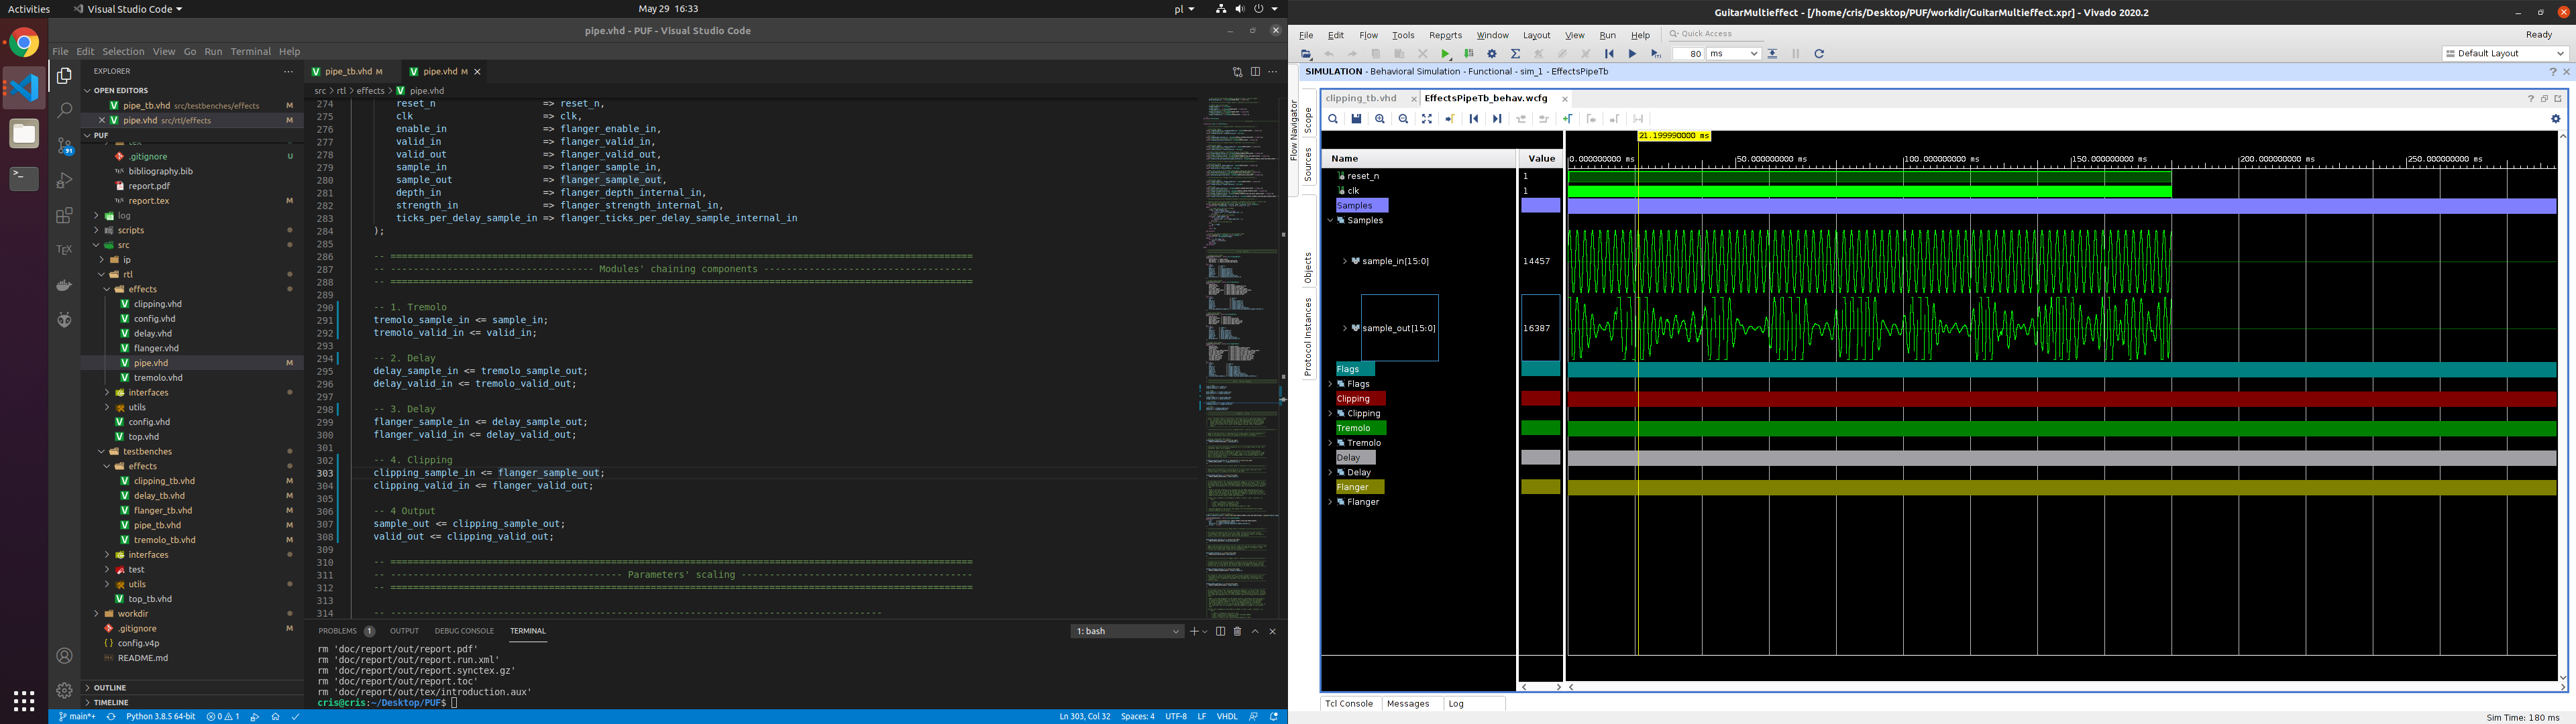
\includegraphics[width=\textwidth]{img/sim/pipe_sim.png}
    \captionsetup{format=plain,justification=centering}
    \caption{Fragment symulacji działania ostatecznego potoku efektów}
    \label{sim-pipe}
\end{figure}
\vspace{0.5cm}
